\documentclass[border=5pt]{standalone}
\usepackage{tikz}
\usepackage{amsmath}
\begin{document}
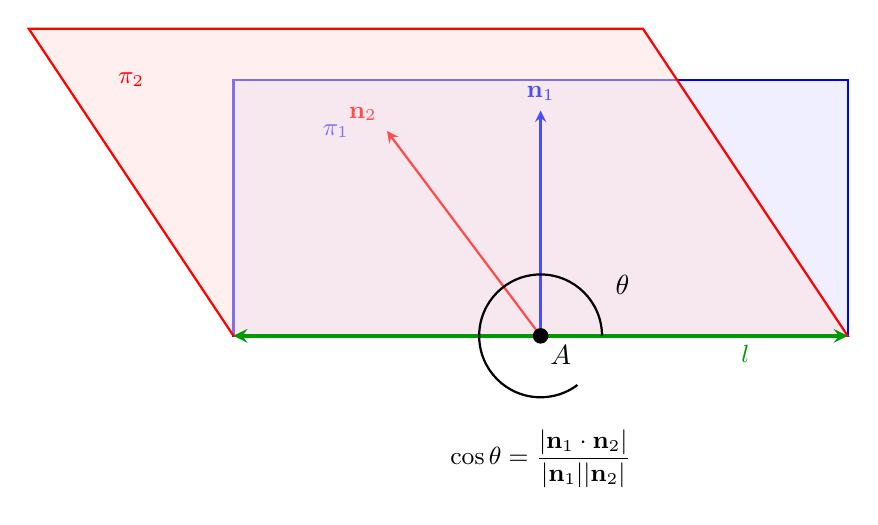
\begin{tikzpicture}[scale=1.3, >=stealth]
  % Angle between two planes

  % Plane 1
  \fill[blue!12, opacity=0.5] (-3,0) -- (3,0) -- (3,2.5) -- (-3,2.5) -- cycle;
  \draw[thick, blue] (-3,0) -- (3,0) -- (3,2.5) -- (-3,2.5) -- cycle;
  \node[blue, font=\small] at (-2, 2) {$\pi_1$};

  % Plane 2 (tilted)
  \fill[red!12, opacity=0.5] (-3,0) -- (3,0) -- (1,3) -- (-5,3) -- cycle;
  \draw[thick, red] (-3,0) -- (3,0) -- (1,3) -- (-5,3) -- cycle;
  \node[red, font=\small] at (-4, 2.5) {$\pi_2$};

  % Intersection line
  \draw[very thick, green!60!black, <->] (-3,0) -- (3,0);
  \node[green!60!black, font=\small, below] at (2, 0) {$l$};

  % Normal vectors from a point on intersection
  \draw[->, thick, blue!70] (0, 0) -- (0, 2.2) node[above, font=\small] {$\mathbf{n}_1$};
  \draw[->, thick, red!70] (0, 0) -- (-1.5, 2.0) node[above left, font=\small] {$\mathbf{n}_2$};

  % Angle between normals
  \draw[thick] (0.6, 0) arc (0:{atan2(2.0,-1.5)+180}:0.6);
  \node at (0.8, 0.5) {$\theta$};

  % Point on intersection
  \filldraw[black] (0, 0) circle (2pt) node[below right] {$A$};

  % Formula
  \node[font=\small] at (0, -1.2) {$\cos\theta = \dfrac{|\mathbf{n}_1\cdot\mathbf{n}_2|}{|\mathbf{n}_1||\mathbf{n}_2|}$};
\end{tikzpicture}
\end{document}
